\section{A closed-form account of the time, and its registered tests}\label{app:relation}
This appendix holds the account of the deployed cache's time that the main text summarises in one paragraph (\cref{sec:gap}): what it is, how it was found, how it fared in the tests registered on machines new to it, and the split of the time it implies. The measured decomposition of \cref{sec:gap} does not rely on it.

\subsection{The relation}
For the deployed cache, we describe the time per token $T$ by
\begin{equation}
T \;=\; G + \frac{\big(M + (1 - G/T)\,A\big)\,S}{B_{\mathrm{host}}},
\label{eq:sum}
\end{equation}
solved for $T$: it is the larger root of $T^2-(G+t_M+t_A)\,T+t_A G=0$, with $t_M=MS/B_{\mathrm{host}}$ and
$t_A=AS/B_{\mathrm{host}}$. $M$ and $A$ are the misses and the background admissions per token (the engine's counters), $S$ the
expert's bytes, $B_{\mathrm{host}}$ the machine's best probed rate, and $G$ the GPU's own kernel time per token in an
Nsight profile of the same engine (\slGprofMin--\slGprofMax\,ms for gpt-oss; where a machine was not profiled or its profile captured no
decode kernels, the median of a fixed set of \jmFallbackHosts{} profiles; \cref{app:more}). $G$ exceeds $T_{\text{GPU}}$ of
\cref{eq:demand} because it also counts the expert kernels the GPU runs for resident and fetched experts. No constant is
fitted to the times. Every
host read costs host time, except the background copies that run while the GPU computes: they spread over the next step,
and a share $G/T$ of them falls under the GPU's compute. The \emph{plain} form drops that share. We found the plain form
on \slLawN{} launches of gpt-oss (exploratory): it is within 6\% on \slLawWithinLow{} of them at 11\% but over-predicts at
25\%, where admissions are a larger share of the reads. The overlap term came from where those copies run, after the
plain form failed its first registered test; over \slOlN{} launches it brings \slOlWithinMid{} instead of
\slPlWithinMid{} within 6\% at 25\%, at the cost of \slOlWithinLow{} instead of \slPlWithinLow{} at 11\%.

\subsection{Registered tests}
After the plain form failed, we registered \cref{eq:sum} before \rtLaterN{} more experiments, each predicting it within a band at every cell, with
$G$ profiled on each machine before its timed runs (\cref{tab:regtests}). None passed as registered.

% the four registered tests of eq. (sum); every value is a macro generated by scripts/job105.py to job108.py
\begin{table}[t]\centering\footnotesize
\caption{The four registered tests of \cref{eq:sum} (job 105: its plain form). A cell is one model and budget on one
machine; \emph{within}: cells where the prediction is within 6\% of the measured time. Each test also registered a pooled
median error of at most 4\%; job 108 registered an 8\% band (\jmWithinEight{} of \jmCells{} cells within it). Jobs 107 and 108 count their valid machines only.}\label{tab:regtests}
\setlength\tabcolsep{3pt}
\begin{tabular}{@{}llrrl@{}}\toprule
Job & Machines new to the test & Within & Median & Outcome \\\midrule
105 & EPYC 7402P, TR 9960X & \jlRegFiveWithin/\jlRegFiveCells & \jgErrMed\% & failed at gpt-oss 25\% \\
106 & EPYC 7302, Xeon 8347C & \jlRegSixWithin/\jlRegSixCells & \jiErrMedAll\% & failed on new machines \\
107 & Ryzen 9 5900XT, AMD ES & \jlWithin/\jlCells & \jlErrMed\% & failed; too few valid \\
108 & EPYC 7543, R9 9950X3D, R9 5950X & \jmWithinSix/\jmCells & \jmErrMed\% & failed (8\% band; EPYC) \\
\bottomrule\end{tabular}
\end{table}


\paragraph{The first test: held on machines rented before, failed on new ones.} On new runs of \jiStable{} machines we had rented before, it came within 6\% at
all \jiCells{} cells of both models (median error \jiErrMed\%). This does not single out the overlap term: discounting
admissions by half passes \jiAltHalf{} of those cells. The same test failed on the two server machines new to it, by
\jiUnstErrMin--\jiUnstErrMax\%; one computed wrong outputs and the other ran its rounds \jiUnstableSpreadMax\% apart (slowest over fastest), so
the following tests set validity gates before launch (\cref{app:more}).

\paragraph{Machines never rented before: not passed.} The next test admitted only machines whose GPU no earlier launch
had recorded, with little host memory in use, correct outputs and rounds within 2\% of each other. Only \jlValidWord{}
of \jlLaunched{} passed, short of the three required, so by its own rule the test is inconclusive; the relation missed the
band at \jlFailCells{} of their \jlCells{} cells, by up to \jlNewServErrMax\% on a dual-socket server
(\rbServSecondMax\% against the probe's second-highest reading) and \jlNewDeskErrMax\% on a Ryzen 9 5900XT. A last test
restricted the machines in advance to the class the relation had been found on (one NUMA node, at most \jlClassCores{}
usable cores) and widened the band to 8\%. It failed on an EPYC 7543 inside that class, by \jmErraLow\%, and without
that machine still failed two pooled clauses (\cref{app:more}).

\paragraph{The error depends on the budget.} On the \jmNewConsWord{} consumer machines new to the last two tests the
relation under-predicted every gpt-oss cell. Over all \rbErrMachines{} consumer machines its mean error is \rbErrMean\%
at gpt-oss 11\% (95\% interval over machines \rbErrLo{} to \rbErrHi) and +\rbErrMidMean\% at 25\% (\rbErrMidLo{} to
\rbErrMidHi): what \cref{eq:sum} leaves out changes sign with the budget.

\subsection{After the fact: the processor}
The processor separates most of the machines the relation fits from those it misses, not all; we drew this split
after the tests. On \jmConsN{} valid launches on \jmConsMachines{} machines with consumer processors, the read rate the deployed
cache implies, $(M + (1-G/T)A)\,S/(T-G)$, is \jmConsEffMin--\jmConsEffMax{} of the probe's best rate at gpt-oss 11\%,
and the relation is within 8\% on \jmConsWithinEight{} of them ($G$ was profiled on the machine for \rbConsProf{} of
these launches). On server processors, \jmServInvalid{} of \jmServAll{}
launches failed a validity check, and the \jmServWord{} valid ones read at \jmServList{} of it: the last fits the
relation, the other two do not. We have not established why. On the dual-socket server the probe's own threads read slower with \jlServCpuManyThreads{} threads, about the
engine's \jlServHelpers{} helpers, than with \jlServCpuBestThreads{} (\jlServCpuMany{} against \jlServCpuBest\,GB/s), and
on an EPYC 9655 rented earlier the per-layer timers showed a latency floor no consumer machine has (the supplement).

\subsection{The split it implies (exploratory)}
On consumer processors, then, the relation splits the deployed cache's time into three parts (\cref{fig:decomp}). At gpt-oss 11\%
the GPU's compute takes \dcShareGLowMin--\dcShareGLowMax\% of the time, MIN's reads, which are the bound,
\dcShareMinLowMin--\dcShareMinLowMax\%, and the reads beyond MIN's \dcShareExLowMin--\dcShareExLowMax\%. The first is
serialisation, the GPU's compute in series with the reads, and makes up \dcGapGLowMin--\dcGapGLowMax\% of the gap to
\cref{eq:limit}; the second is the reads MIN would not make. With $G$ removed, the time scales with the host's read rate
with an elasticity of \slElastLow{} (95\% interval \slElastLowLo{} to \slElastLowHi{} over the machines of the
exploratory set), as reads at
$B_{\mathrm{host}}$ would. Foresight can attack both parts: fewer reads need MIN's choices, and overlap needs reads
issued ahead. Reading below the probed rate takes at most \dcDeskShortLowMax\% of the time on the consumer machines;
on the server machines it is a third part (\dcServShortLow{} of the time at 11\%).

\begin{figure*}[t]\centering
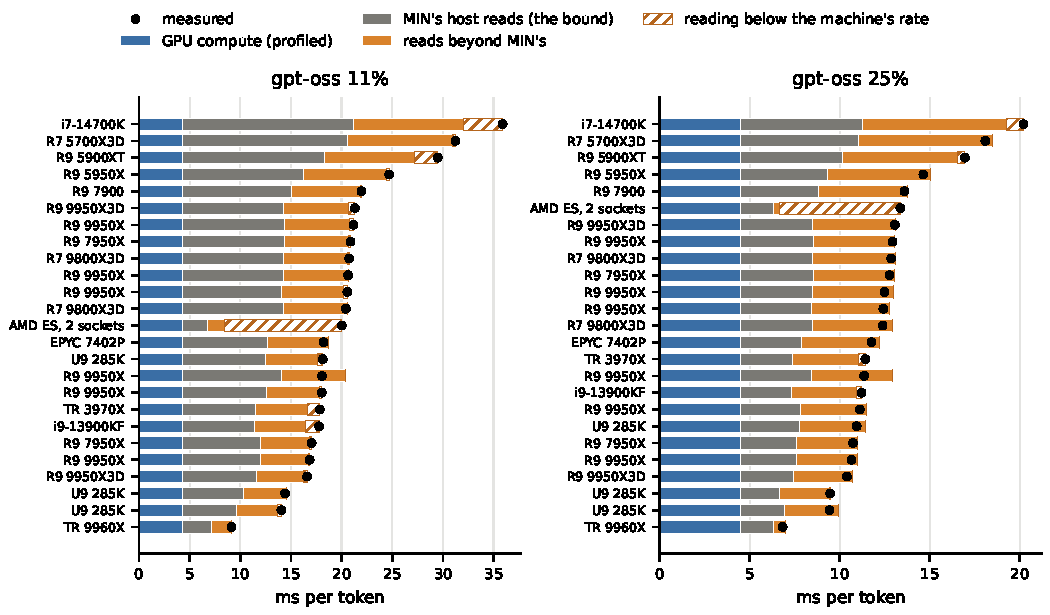
\includegraphics[width=\textwidth]{figs/decomp.pdf}
\caption{Where the seconds go, machine by machine: the deployed cache's time per token at the two host-bound gpt-oss
budgets split by \cref{eq:sum} into the GPU's compute ($G$, profiled on the machine, or the median profile where none
was taken or it captured no decode kernels), MIN's host reads at the machine's best rate (the bound of \cref{eq:limit}) and the reads the cache makes
beyond MIN's. The dot is the measured time; hatched, the measured time beyond \cref{eq:sum}, reading below the machine's
best rate; a bar that ends past the dot is an over-prediction. Machines with the same processor are numbered in order of
rental. One launch per machine that ran stably: \dcMachinesLow{} with consumer processors (above the dashed line)
and \dcServLowN{} with server processors (below). $^*$: first rented for a registered test of \cref{eq:sum}.}
\label{fig:decomp}
\end{figure*}

